\author{Oliver Wallscheid}
\part{Lecture 09: On-Policy Prediction with Function Approximation}
\title[RL Lecture 09]{Lecture 09: On-Policy Prediction \\with Function Approximation}  
\date{}  
\frame{\titlepage} 

%%%%%%%%%%%%%%%%%%%%%%%%%%%%%%%%%%%%%%%%%%%%%%%%%%%%%%%%%%%%%
%% Preface %%
%%%%%%%%%%%%%%%%%%%%%%%%%%%%%%%%%%%%%%%%%%%%%%%%%%%%%%%%%%%%%
\frame{\frametitle{Preface}
Until further notice we assume that:
\begin{itemize}
	\item The \hl{state space is consisting of at least one continuous quantity or an unfeasible large amount of discrete states (quasi-continuous)}.
	\begin{itemize}
		\item The state is considered a vector: $\bm{x}=\begin{bmatrix} x_1 & x_2 & \cdots \end{bmatrix}\T$ .\pause
	\end{itemize}
	\item The \hl{action space remains discrete and feasible small}.
	\begin{itemize}
		\item The action can be represented as a scalar: $\bm{u}=u$ (cf. 2nd lecture). \pause
	\end{itemize}
	\item The applied approximation tools are \hl{differentiable functions} $J(\bm{w})$ with the parameter vector $\bm{w}$.
	\begin{itemize}
		\item Therefore, the gradient $\nabla J(\bm{w})=\begin{bmatrix} \frac{\partial J(\bm{w})}{\partial w_1} & \frac{\partial J(\bm{w})}{\partial w_2} & \cdots \end{bmatrix}\T$ exists. \pause
	\end{itemize}
\end{itemize}
Focus of this and the next lecture:
\begin{itemize}
	\item Transferring previous RL methods from discrete to continuous state-space problems in the on-policy case.\pause
	\item Applying off-policy approaches with function approximation is not straightforward and will be largely skipped.  
	\begin{itemize}
		\item For further insights we refer to chapter 11 in \textit{R. Sutton and G. Barto, Reinforcement learning: an introduction, 2018}. 
	\end{itemize}
\end{itemize}
}

%%%%%%%%%%%%%%%%%%%%%%%%%%%%%%%%%%%%%%%%%%%%%%%%%%%%%%%%%%%%%%%%%%
\section{Impact of Function Approximation to the RL Task} 
%%%%%%%%%%%%%%%%%%%%%%%%%%%%%%%%%%%%%%%%%%%%%%%%%%%%%%%%%%%%%%%%%%
\begin{frame}
\frametitle{Table of Contents}
\tableofcontents
\end{frame}

%%%%%%%%%%%%%%%%%%%%%%%%%%%%%%%%%%%%%%%%%%%%%%%%%%%%%%%%%%%%%
%% Non-stationarity  %%
%%%%%%%%%%%%%%%%%%%%%%%%%%%%%%%%%%%%%%%%%%%%%%%%%%%%%%%%%%%%%
\frame{\frametitle{Non-stationarity}
\begin{itemize}
	\item Standard assumption of supervised ML: static and i.i.d. data processes \pause
	\item Deviating impacts in the RL framework:
	\begin{itemize}
		\item Changing environments (e.g. by tear and wear)
		\item Dynamic learning in control tasks i.e. changing policy (next lecture)
	\end{itemize}
\end{itemize}
\begin{figure}
	\subfloat{
		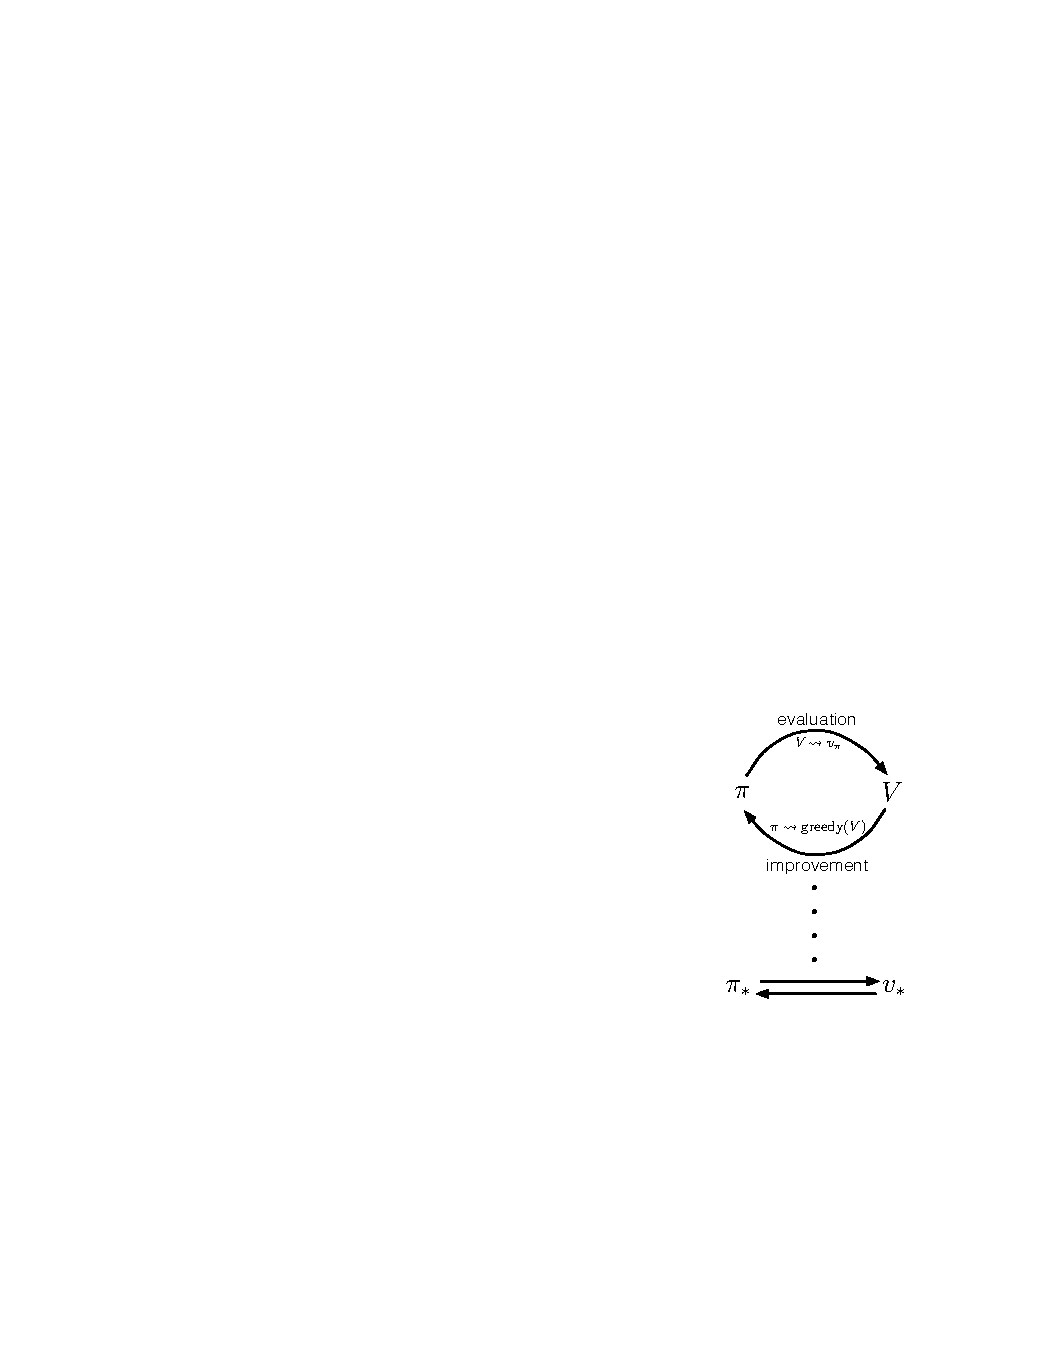
\includegraphics[height=3.8cm]{fig/lec03/GPI_01.pdf}
	}
	\hspace{1cm}
	\subfloat{
		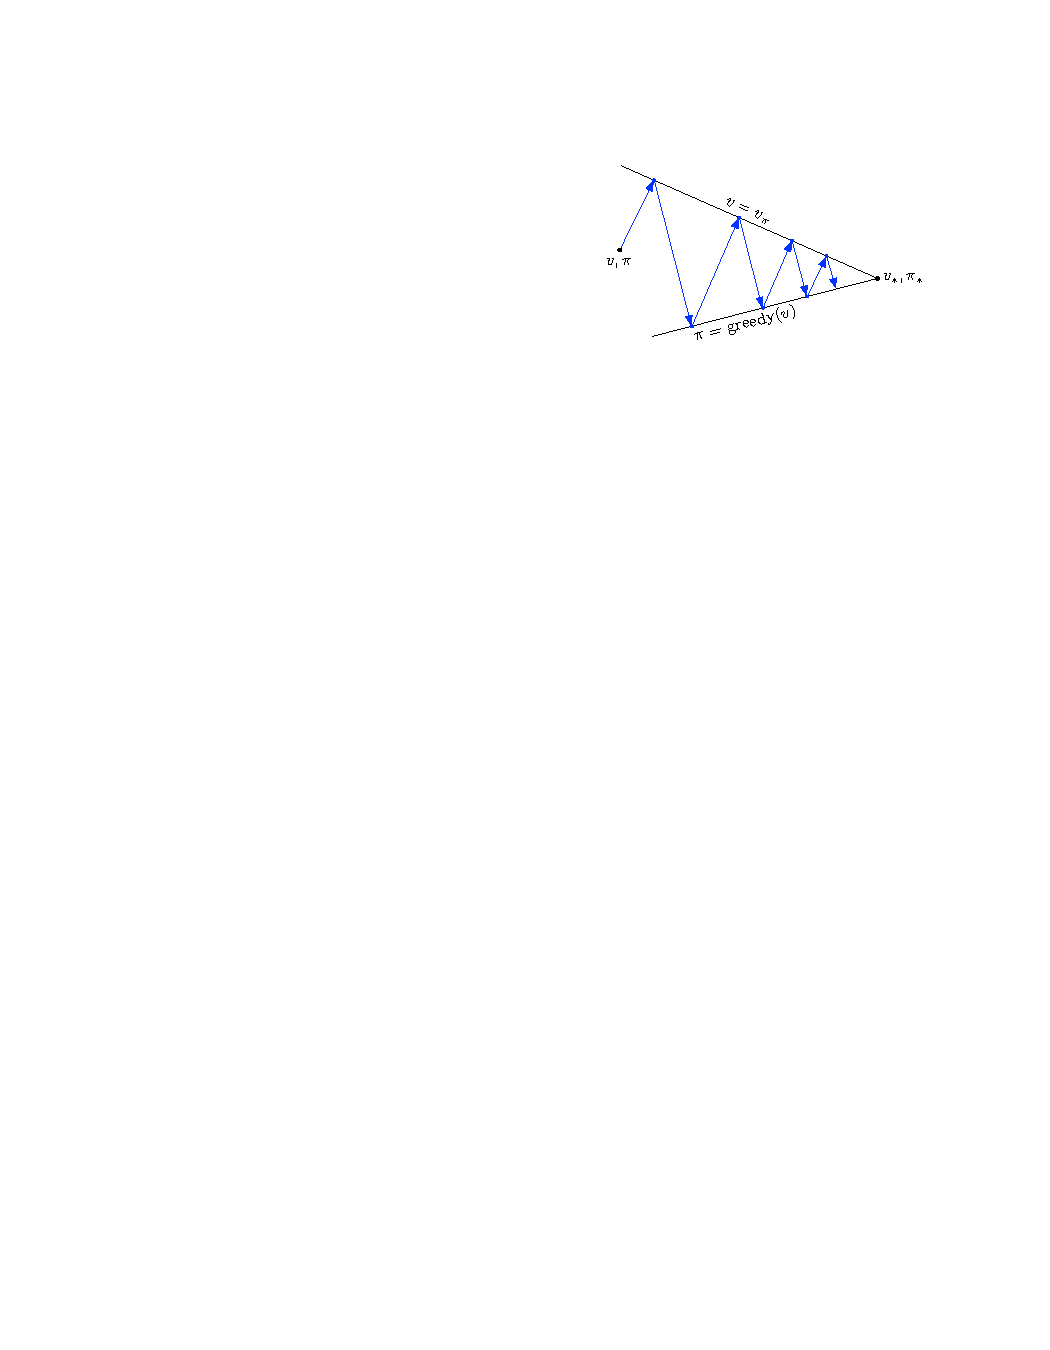
\includegraphics[height=3.8cm]{fig/lec03/GPI_02.pdf}
	}
\caption{GPI changes the underlying stochastic processes generating data inputs to be learned by function approximators (source: R. Sutton and G. Barto, Reinforcement learning: an introduction, 2018, \href{https://creativecommons.org/licenses/by-nc-nd/2.0/}{CC BY-NC-ND 2.0})}
\end{figure}
}


%%%%%%%%%%%%%%%%%%%%%%%%%%%%%%%%%%%%%%%%%%%%%%%%%%%%%%%%%%%%%
%% Prediction Objective with Function Approximation (1)%%
%%%%%%%%%%%%%%%%%%%%%%%%%%%%%%%%%%%%%%%%%%%%%%%%%%%%%%%%%%%%%
\frame{\frametitle{Prediction Framework with Function Approximation (1)}
\begin{itemize}
	\item Estimate true value function $v_\pi(\bm{x})$ using a parametrizable approximate value function
		\begin{equation}
			\hat{v}(\tilde{\bm{x}}, \bm{w}) \approx v_\pi(\bm{x}) .
		\end{equation}
	\item The state $\bm{x}$ might be enhanced by \hl{feature engineering} (i.e. additional signal inputs are derived in the \hl{feature vector $\tilde{\bm{x}}=\bm{f}(\bm{x})\in\mathbb{R}^\kappa$}).
	\item Above, \hl{$\bm{w} \in \mathbb R^\zeta$ is the parameter vector}. \pause
	\item Typically, $\zeta << |\mathcal{X}|$ applies (otherwise approximation is pointless).\pause
\end{itemize}
\begin{block}{Generalization}
Due to the usage of function approximation one incremental learning step changes at least one element $w_i\in\bm{w}$ which
\begin{itemize}
	\item affects the estimated value of many states compared to
	\item the tabular case where one update step affects only one state.
\end{itemize}
\end{block}
}

%%%%%%%%%%%%%%%%%%%%%%%%%%%%%%%%%%%%%%%%%%%%%%%%%%%%%%%%%%%%%
%% Prediction Objective with Function Approximation (2)%%
%%%%%%%%%%%%%%%%%%%%%%%%%%%%%%%%%%%%%%%%%%%%%%%%%%%%%%%%%%%%%
\frame{\frametitle{Prediction Framework with Function Approximation (2)}
\begin{itemize}
	\item In the tabular case a specific \hl{prediction objective} was not needed:
	\begin{itemize}
		\item The learned value function could exactly match the true value.
		\item The value estimate at each state was decoupled from other states.  \pause
	\end{itemize}
	\item Due to generalization impact we need to define an accuracy metric on the entire state space (the RL prediction goal):
\end{itemize}
\begin{defi}{Mean Squared Value Error}{VE}
The RL prediction objective is defined as the mean squared value error
\begin{equation}
	\overline{\mbox{VE}}(\bm{w}) = \int_{\mathcal{X}}\mu(\bm{x})\left[v_{\pi}(\bm{x}) - \hat{v}(\tilde{\bm{x}}, \bm{w})\right]^2
\label{eq:VE}
\end{equation}
with $\mu(\bm{x})\in\left\{\mathbb{R}|\mu(\bm{x})\geq 0\right\}$ being a state distribution weight with $\int_{\mathcal{X}}\mu=1$. 
\end{defi}\pause
\begin{itemize}
	\item Practical note: As the true value $v_{\pi}(\bm{x})$ is most likely unknown in most tasks, \eqref{eq:VE} cannot be computed exactly but only estimated.
\end{itemize}
}

%%%%%%%%%%%%%%%%%%%%%%%%%%%%%%%%%%%%%%%%%%%%%%%%%%%%%%%%%%%%%
%% Simplification for On-Policy Prediction %%
%%%%%%%%%%%%%%%%%%%%%%%%%%%%%%%%%%%%%%%%%%%%%%%%%%%%%%%%%%%%%
\frame{\frametitle{Simplification for On-Policy Prediction}
\begin{itemize}
	\item For prediction we focus entirely on the on-policy case. 
	\item Hence, \hl{$\mu(\bm{x})$ is the on-policy distribution} under $\pi$. \pause
	\item For practical usage we can therefore approximate the weighted integration over the entire state space $\mathcal{X}$ in \eqref{eq:VE} by the sampled MSE of the visited state trajectory:
\end{itemize}
\vspace{0.5cm}
\begin{equation}
	\overline{\mbox{VE}}(\bm{w}) \approx J(\bm{w})= \sum_k \left[v_{\pi}(\bm{x}_k) - \hat{v}(\tilde{\bm{x}}_k, \bm{w})\right]^2
\label{eq:VE_J}
\end{equation}\pause
\vspace{0.25cm}
\begin{itemize}
	\item If we would perform off-policy prediction we have to transform the sampled value (estimates) from the behavior to the target policy.
	\item Likewise when doing this for tabular methods, this increases the prediction variance. \pause
	\item In combination with generalization errors due to function approximation, the overall risk of diverging is significantly higher compared to the on-policy case.
\end{itemize}
}


%%%%%%%%%%%%%%%%%%%%%%%%%%%%%%%%%%%%%%%%%%%%%%%%%%%%%%%%%%%%%
%% Prediction Challenges with Function Approximation %%
%%%%%%%%%%%%%%%%%%%%%%%%%%%%%%%%%%%%%%%%%%%%%%%%%%%%%%%%%%%%%
\frame{\frametitle{Prediction Challenges with Function Approximation}
Summarizing the two previous slides:
\begin{itemize}
	\item The goal is to find 
	\begin{equation}
		\bm{w}^* = \argmin_{\bm{w}} J(\bm{w}).
		\label{eq:min_prediction_objective}
	\end{equation}
\end{itemize}\pause
First challenge:
\begin{itemize}
	\item Function approximator $\hat{v}(\tilde{\bm{x}}, \bm{w})$ requires certain form to fit $v_{\pi}(\bm{x})$.
\end{itemize}\pause
\vspace{0.5cm}
Second challenge:
\begin{itemize}
	\item If $\hat{v}(\tilde{\bm{x}}, \bm{w})$ is linear: convex optimization problem.
	\begin{itemize}
		\item The \hl{nice case}: the local optimum equals the global optimum and is uniquely discoverable. But requires linear feature dependence.
	\end{itemize}\pause
	\item If $\hat{v}(\tilde{\bm{x}}, \bm{w})$ is non-linear: non-linear optimization problem.
	\begin{itemize}
		\item The \hl{ugly case}: possible multitude of local optima with no guarantee to locate the global one. 
		\item Depending on optimization strategy the \hl{RL algorithm may diverge}. 
	\end{itemize}
\end{itemize}
}

%%%%%%%%%%%%%%%%%%%%%%%%%%%%%%%%%%%%%%%%%%%%%%%%%%%%%%%%%%%%%%%%%%
\section{Gradient-Based Prediction} 
%%%%%%%%%%%%%%%%%%%%%%%%%%%%%%%%%%%%%%%%%%%%%%%%%%%%%%%%%%%%%%%%%%
\begin{frame}
\frametitle{Table of Contents}
\tableofcontents[currentsection]
\end{frame}

%%%%%%%%%%%%%%%%%%%%%%%%%%%%%%%%%%%%%%%%%%%%%%%%%%%%%%%%%%%%%
%% Updating the Parameter Vector to Find (Local) Optimum %%
%%%%%%%%%%%%%%%%%%%%%%%%%%%%%%%%%%%%%%%%%%%%%%%%%%%%%%%%%%%%%
\frame{\frametitle{Updating the Parameter Vector to Find (Local) Optimum}
Transferring the idea of incremental learning steps from the tabular case 
\begin{equation}
	\hat{v}(x) \leftarrow \hat{v}(x) + \alpha \left[v_\pi(x) - \hat{v}(x)\right] 
\end{equation}
to function approximation using a gradient descent update:
\begin{equation}
	\bm{w}\leftarrow\bm{w}-\alpha \nabla_{\bm{w}}J(\bm{w}).
	\label{eq:gradient_learning}
\end{equation}
\begin{itemize}
	\item The search direction is the prediction objective gradient $\nabla_{\bm{w}}J(\bm{w})$.
	\item The learning rate $\alpha$ determines the step size of one update.
\end{itemize}
}

%%%%%%%%%%%%%%%%%%%%%%%%%%%%%%%%%%%%%%%%%%%%%%%%%%%%%%%%%%%%%
%% How to Retrieve the Gradient? %%
%%%%%%%%%%%%%%%%%%%%%%%%%%%%%%%%%%%%%%%%%%%%%%%%%%%%%%%%%%%%%
\frame{\frametitle{How to Retrieve the Gradient?}
\begin{columns}[t,onlytextwidth]
\begin{column}{0.475\textwidth}
\begin{minipage}[c]{\linewidth}
\begin{figure}
	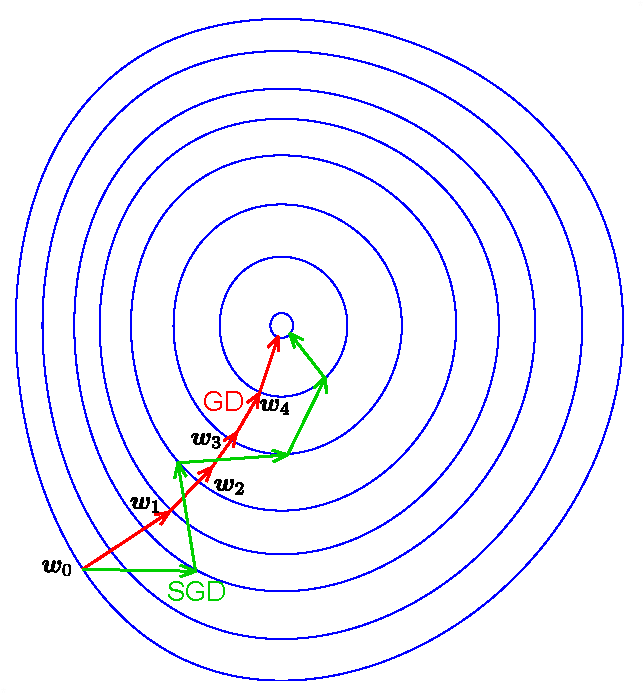
\includegraphics[width=4.5cm]{fig/lec09/Gradient_descent.pdf}
	\caption{Exemplary optimization paths for (stochastic) gradient descent \\(derivative work of \href{https://commons.wikimedia.org/wiki/File:Gradient_descent.svg}{www.wikipedia.org}, \href{https://creativecommons.org/publicdomain/zero/1.0/deed.en}{CC0 1.0})}
	\label{fig:Gradient_descent}
\end{figure}
\end{minipage}
\end{column}
\hfill
\begin{column}{0.54\textwidth}
\begin{minipage}[c]{\linewidth}
\begin{itemize}
	\item Full calculus of $\nabla_{\bm{w}}J(\bm{w})$:
	\begin{itemize}
		\item Batch evaluation on sampled sequence $\bm{x}_0, \bm{x}_1, \bm{x}_2,\ldots$ might be computationally costly. 
		\item In RL control: since $\pi$ changes over time, past data in batch is not fully representative. 
	\end{itemize}\pause
	\item SGD: sample gradient at a given state $\bm{x}_k$ and parameter vector $\bm{w}_k$:
	\begin{equation*}
	\begin{split}
		\nabla_{\bm{w}}J(\bm{w}) \approx &-\left[v_\pi(\bm{x}_k) - \hat{v}(\tilde{\bm{x}}_k, \bm{w}_k)\right]\\ &\hspace{0.1cm}\nabla_{\bm{w}} \hat{v}(\tilde{\bm{x}}_k, \bm{w}_k).
	\end{split}
	\end{equation*}\pause
	\item Regular gradient descent leads to same result as SGD in expectation (averaging of samples). 
\end{itemize}
\end{minipage}
\end{column}
\end{columns}
}

%%%%%%%%%%%%%%%%%%%%%%%%%%%%%%%%%%%%%%%%%%%%%%%%%%%%%%%%%%%%%
%% Asking an Expert on Convergence Properties %%
%%%%%%%%%%%%%%%%%%%%%%%%%%%%%%%%%%%%%%%%%%%%%%%%%%%%%%%%%%%%%
\frame{\frametitle{Asking an Expert on Convergence Properties}
The optimization task \eqref{eq:min_prediction_objective} could be
\begin{itemize}
	\item non-linear,
	\item multidimensional and
	\item non-stationary.
\end{itemize}\pause
Applying gradient descent to such a problem requires:
\begin{itemize}
	\item Enormous luck to initialize $\bm{w}_0$ close to the global optimum.
	\item Cautious tuning of $\alpha$ to prevent diverging or chattering of $\bm{w}_k$.
\end{itemize}
\begin{figure}
	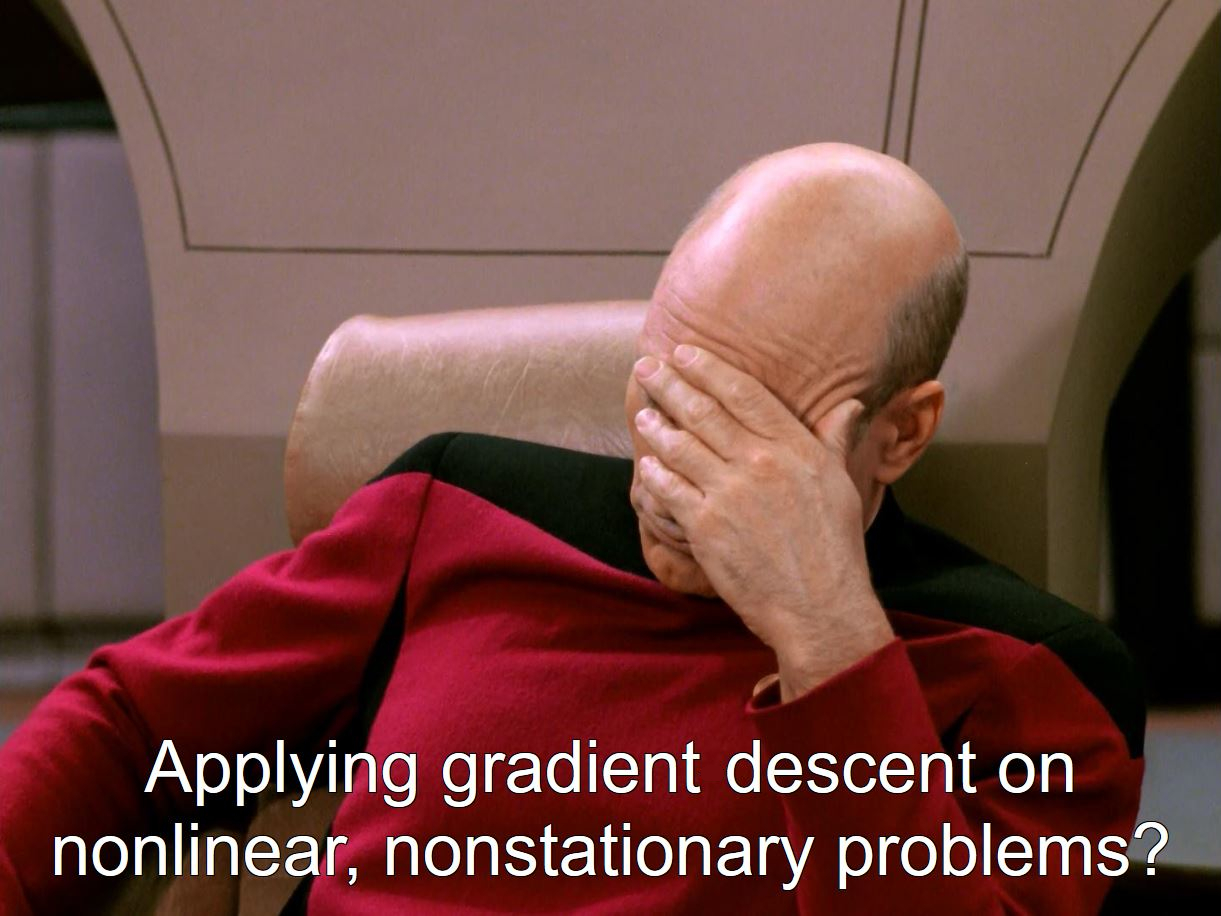
\includegraphics[width=6cm]{fig/lec09/Picard_GD.jpg}
	\label{fig:Picard_GD.jpg}
\end{figure}
}

%%%%%%%%%%%%%%%%%%%%%%%%%%%%%%%%%%%%%%%%%%%%%%%%%%%%%%%%%%%%%
%% SGD-Based Learning Step %%
%%%%%%%%%%%%%%%%%%%%%%%%%%%%%%%%%%%%%%%%%%%%%%%%%%%%%%%%%%%%%
\frame{\frametitle{SGD-Based Learning Step}
Despite the possible problems we apply SGD-based learning due to its striking simplicity (and wide distribution in the literature): 
\begin{block}{Gradient-based parameter update}
To optimize \eqref{eq:min_prediction_objective} by an appropriate function approximator $\hat{v}(\tilde{\bm{x}}, \bm{w})$ the incremental learning update per step is
 \begin{equation}
	 \bm{w}_{k+1} = \bm{w}_{k} + \alpha\left[v_\pi(\bm{x}_k) - \hat{v}(\tilde{\bm{x}}_k, \bm{w}_k)\right]\nabla_{\bm{w}} \hat{v}(\tilde{\bm{x}}_k, \bm{w}_k) .
	\label{eq:gradient_param_value}
 \end{equation}
\end{block}\pause
Nevertheless, the true update target $v_\pi(\bm{x}_k)$ is often unknown due to
\begin{itemize}
	\item noise or
	\item the learning process itself (e.g. bootstrapping estimates). 
\end{itemize}
}

%%%%%%%%%%%%%%%%%%%%%%%%%%%%%%%%%%%%%%%%%%%%%%%%%%%%%%%%%%%%%
%% Generalization Example for Gradient-Based Parameter Update %%
%%%%%%%%%%%%%%%%%%%%%%%%%%%%%%%%%%%%%%%%%%%%%%%%%%%%%%%%%%%%%
\frame{\frametitle{Generalization Example for Parameter Update}
\begin{itemize}
	\item Function approximation $\hat{v}(\tilde{\bm{x}}, \bm{w})=\begin{bmatrix}w_1 & w_2 & w_3\end{bmatrix}\begin{bmatrix}x_1 & x_2 & 1\end{bmatrix}\T$\pause
	\item Initial parameter: $\bm{w}\T_0=\begin{bmatrix}1 & 1 & 1\end{bmatrix}$, $v_\pi(\bm{x}_0=\begin{bmatrix}1 & 1\end{bmatrix}\T)=1$,  $\alpha=0.1$\pause
	\item New parameter set:
	\begin{align*}
	\bm{w}\T_{1} 		&= \bm{w}\T_{0} + \alpha\left[v_\pi(\bm{x}_0) - \hat{v}(\tilde{\bm{x}}_0, \bm{w}_0)\right](\nabla_{\bm{w}} \hat{v}(\tilde{\bm{x}}_0, \bm{w}_0))\T\\
								&=\begin{bmatrix}1 & 1 & 1\end{bmatrix} + 0.1\left(1-3\right)\begin{bmatrix}1 & 1 & 1\end{bmatrix}=\begin{bmatrix}0.8 & 0.8 & 0.8\end{bmatrix}
 \end{align*}
\end{itemize}
\pause
\begin{figure}
	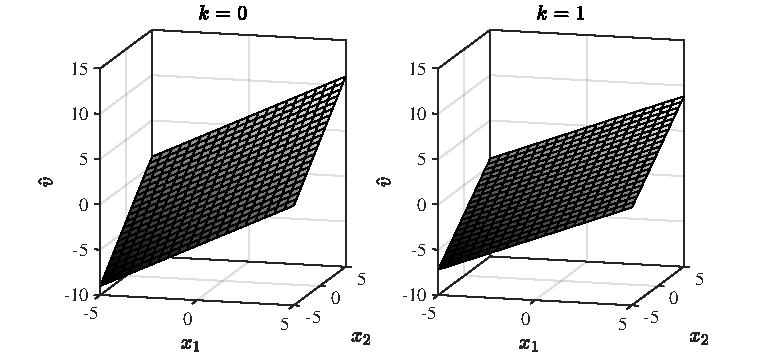
\includegraphics[width=9.25cm]{fig/lec09/Simple_LinearRegression_Example.pdf}
	\label{fig:Simple_LinearRegression_Example.jpg}
	\caption{Exemplary state-value estimation update with linear regression model}
\end{figure}
}

%%%%%%%%%%%%%%%%%%%%%%%%%%%%%%%%%%%%%%%%%%%%%%%%%%%%%%%%%%%%%
%% Gradient Monte Carlo %%
%%%%%%%%%%%%%%%%%%%%%%%%%%%%%%%%%%%%%%%%%%%%%%%%%%%%%%%%%%%%%
\frame{\frametitle{Algorithmic Implementation: Gradient Monte Carlo}
\begin{itemize}
	\item Direct transfer from tabular case to function approximation
	\item Update target becomes the sampled return $v_\pi(\bm{x}_k)\approx g_k$
\end{itemize}
\setlength{\algomargin}{0.5em}
\begin{algorithm}[H]
\SetKwInput{Input}{input} 
\SetKwInput{Output}{output}
\SetKwInput{Init}{init}
\SetKwInput{Param}{parameter}
\Input{a policy $\pi$ to be evaluated, a feature representation $\tilde{\bm{x}}=\bm{f}(\bm{x})$}
\Input{a differentiable function $\hat{v}:\mathbb{R}^\kappa\times\mathbb{R}^\zeta\rightarrow\mathbb{R}$}
\Param{step size $\alpha\in\left\{\mathbb{R}|0<\alpha<1\right\}$}
\Init{value-function weights $\bm{w}\in\mathbb{R}^\zeta$ arbitrarily}
 \For{$j=1,2,\ldots,$ episodes}{
		generate an episode following $\pi$: $x_{0}, u_{0}, r_{1},\ldots,x_{T}$ \;
		calculate every-visit return $g_k$\;  
		\For{$k=0,1,\ldots, T-1$ time steps}{
			$\bm{w} \leftarrow \bm{w} + \alpha\left[g_k - \hat{v}(\tilde{\bm{x}}_k, \bm{w})\right]\nabla_{\bm{w}} \hat{v}(\tilde{\bm{x}}_k, \bm{w})$\; 
		}
	}
\caption{Every-visit gradient MC (output: parameter vector $\bm{w}$ for $\hat{v}_\pi$)}
\label{algo:MC_gradient}
\end{algorithm}
}

%%%%%%%%%%%%%%%%%%%%%%%%%%%%%%%%%%%%%%%%%%%%%%%%%%%%%%%%%%%%%
%% Semi-Gradient Methods %%
%%%%%%%%%%%%%%%%%%%%%%%%%%%%%%%%%%%%%%%%%%%%%%%%%%%%%%%%%%%%%
\frame{\frametitle{Semi-Gradient Methods}
\begin{itemize}
	\item If bootstrapping is applied, the true target $v_\pi(\bm{x}_k)$ is approximated by a target depending on the estimate $\hat{v}(\tilde{\bm{x}}_k, \bm{w})$.\pause
	\item If $\hat{v}(\tilde{\bm{x}}_k, \bm{w})$ does not perfectly fit  $v_\pi(\bm{x}_k)$, \hl{the update target becomes a biased estimate of $v_\pi(\bm{x}_k)$}.\pause
	\begin{itemize}
		\item For example, in the TD(0) case applying SGD we receive: 
		\end{itemize}
		\begin{equation}
		\begin{split}
				v_\pi(\bm{x}) &\approx r + \gamma \hat{v}(\tilde{\bm{x}}', \bm{w}),\\
				J(\bm{w}) &\approx \sum_k \left[r_{k+1} + \gamma \hat{v}(\tilde{\bm{x}}_{k+1}, \bm{w}_k) - \hat{v}(\tilde{\bm{x}}_k, \bm{w}_k)\right]^2,\\
				\nabla_{\bm{w}} J(\bm{w}) &\approx \left[r_{k+1} + \gamma \hat{v}(\tilde{\bm{x}}_{k+1}, \bm{w}_k) - \hat{v}(\tilde{\bm{x}}_k, \bm{w}_k)\right]\\
				&\hspace{0.5cm}\nabla_{\bm{w}} \left[\gamma \hat{v}(\tilde{\bm{x}}_{k+1}, \bm{w}_k)  - \hat{v}(\tilde{\bm{x}}_k, \bm{w}_k)\right].
		\end{split}	
		\end{equation}
\end{itemize}\pause
\vspace{-0.2cm}
\begin{block}{Semi-gradient methods}
When bootstrapping is applied, the gradient does not take into account any gradient component of the bootstrapped target estimate.    
\end{block}\pause
\begin{itemize}
	\item Motivation: speed up gradient calculation while assuming that the simplification error is small (e.g. due to discounting).
\end{itemize}
}

%%%%%%%%%%%%%%%%%%%%%%%%%%%%%%%%%%%%%%%%%%%%%%%%%%%%%%%%%%%%%
%% Semi-Gradient TD(0) %%
%%%%%%%%%%%%%%%%%%%%%%%%%%%%%%%%%%%%%%%%%%%%%%%%%%%%%%%%%%%%%
\frame{\frametitle{Algorithmic Implementation: Semi-Gradient TD(0)}
The semi-gradient of $J(\bm{w})$ for TD(0) from prev. slide is then
\begin{equation}
	\nabla_{\bm{w}} J(\bm{w}) \approx -\left[r_{k+1} + \gamma \hat{v}(\tilde{\bm{x}}_{k+1}, \bm{w}_k) - \hat{v}(\tilde{\bm{x}}_k, \bm{w}_k)\right]\nabla_{\bm{w}}\hat{v}(\tilde{\bm{x}}_k, \bm{w}_k) .
\end{equation}\pause
\setlength{\algomargin}{0.5em}
\begin{algorithm}[H]
\SetKwInput{Input}{input} 
\SetKwInput{Output}{output}
\SetKwInput{Init}{init}
\SetKwInput{Param}{parameter}
\Input{a policy $\pi$ to be evaluated, a feature representation $\tilde{\bm{x}}=\bm{f}(\bm{x})$}
\Input{a differentiable function $\hat{v}:\mathbb{R}^\kappa\times\mathbb{R}^\zeta\rightarrow\mathbb{R}$ with $\hat{v}(\tilde{\bm{x}}_T, \cdot)=0$}
\Param{step size $\alpha\in\left\{\mathbb{R}|0<\alpha<1\right\}$}
\Init{value-function weights $\bm{w}\in\mathbb{R}^\zeta$ arbitrarily}
 \For{$j=1,2,\ldots$ episodes}{
		initialize $\bm{x}_{0}$\;
		\For{$k=0, 1, 2 \ldots $ time steps}{
			$u_k \leftarrow$ apply action from $\pi(\bm{x}_k)$\;
			observe $\bm{x}_{k+1}$ and $r_{k+1}$\;
			$\bm{w} \leftarrow \bm{w} + \alpha\left[r_{k+1} +\gamma \hat{v}(\tilde{\bm{x}}_{k+1}, \bm{w}) - \hat{v}(\tilde{\bm{x}}_k, \bm{w})\right]\nabla_{\bm{w}} \hat{v}(\tilde{\bm{x}}_k, \bm{w})$\; 
			exit loop if $\bm{x}_{k+1}$ is terminal\;
		}
	}
\caption{Semi-gradient TD(0) (output: parameter vector $\bm{w}$ for $\hat{v}_\pi$)}
\label{algo:Semi_gradient_TD0}
\end{algorithm}
}

%%%%%%%%%%%%%%%%%%%%%%%%%%%%%%%%%%%%%%%%%%%%%%%%%%%%%%%%%%%%%
%% n-step Semi-Gradient TD %%
%%%%%%%%%%%%%%%%%%%%%%%%%%%%%%%%%%%%%%%%%%%%%%%%%%%%%%%%%%%%%
\frame{
\setlength{\algomargin}{0.5em}
\begin{algorithm}[H]
\small
\SetKwInput{Input}{input} 
\SetKwInput{Output}{output}
\SetKwInput{Init}{init}
\SetKwInput{Param}{parameter}
\Input{a policy $\pi$ to be evaluated, a feature representation $\tilde{\bm{x}}= \bm{f}(\bm{x})$}
\Input{a differentiable function $\hat{v}:\mathbb{R}^\kappa\times\mathbb{R}^\zeta\rightarrow\mathbb{R}$ with $\hat{v}(\tilde{\bm{x}}_T, \cdot)=0$}
\Param{step size $\alpha\in\left\{\mathbb{R}|0<\alpha<1\right\}$, prediction steps $n\in\mathbb{Z}^+$}
\Init{value-function weights $\bm{w}\in\mathbb{R}^\zeta$ arbitrarily}
 \For{$j=1,2\ldots$ episodes}{
		initialize and store $\bm{x}_{0}$\;
		$T\leftarrow\infty$\;
		\Repeat( $k=0, 1, 2, \ldots$){$\tau=T-1$}{
			\If{$k<T$}{
				take action from $\pi(\bm{x}_k)$, observe and store $\bm{x}_{k+1}$ and $r_{k+1}$\;
				if $\bm{x}_{k+1}$ is terminal: $T\leftarrow k+1$\;
				}
			$\tau\leftarrow k-n+1$ ($\tau$ time index for estimate update)\;
			\If{$\tau \geq 0$}{
				$g\leftarrow \sum_{i=\tau+1}^{\min(\tau + n, T)}\gamma^{i-\tau-1} r_i$\;
				if $\tau+n < T$: $g\leftarrow g + \gamma^n \hat{v}(\tilde{\bm{x}}_{\tau+n}, \bm{w})$\;
				$\bm{w} \leftarrow \bm{w} + \alpha\left[g - \hat{v}(\tilde{\bm{x}}_\tau, \bm{w})\right]\nabla_{\bm{w}} \hat{v}(\tilde{\bm{x}}_\tau, \bm{w})$\; 
			}
		}
	}
\caption{$n$-step semi-gradient TD (output: parameter vector $\bm{w}$ for $\hat{v}_\pi$)}
\label{algo:Semi_gradient_TD_nstep}
\end{algorithm}
}

%%%%%%%%%%%%%%%%%%%%%%%%%%%%%%%%%%%%%%%%%%%%%%%%%%%%%%%%%%%%%%%%%%
\section{Batch Learning} 
%%%%%%%%%%%%%%%%%%%%%%%%%%%%%%%%%%%%%%%%%%%%%%%%%%%%%%%%%%%%%%%%%%
\begin{frame}
\frametitle{Table of Contents}
\tableofcontents[currentsection]
\end{frame}

%%%%%%%%%%%%%%%%%%%%%%%%%%%%%%%%%%%%%%%%%%%%%%%%%%%%%%%%%%%%%
%% Background and Motivation %%
%%%%%%%%%%%%%%%%%%%%%%%%%%%%%%%%%%%%%%%%%%%%%%%%%%%%%%%%%%%%%
\frame{\frametitle{Background and Motivation}
\begin{itemize}
	\item As already discussed in the tabular case: incremental learning is not data efficient (cf. example \figref{fig:Batch_AB_Example}).
	\begin{itemize}
		\item During one incremental learning step we are not utilizing the given information to the maximum possible extent.
		\item Also applies to SGD-based updates with function approximation.
	\end{itemize}\pause
	\vspace{0.5cm}
	\item Alternative: batch learning methods
	\begin{itemize}
		\item Find $\bm{w}^*$ given a fixed, consistent data set $\bm{\mathcal{D}}$
		\item $\bm{\mathcal{D}}=\left\{\left\langle \bm{x}_0, v_\pi(\bm{x}_0)\right\rangle, \left\langle \bm{x}_1, v_\pi(\bm{x}_1)\right\rangle,\ldots\right\}$
	\end{itemize}\pause
\vspace{0.5cm}
\item What batch learning options do we have?
	\begin{itemize}
		\item Experience replay (cf. planning and learning lecture e.g. \figref{fig:Dyna})
		\item If $\hat{v}(\tilde{\bm{x}}, \bm{w})$ is linear: closed-form least-squares solution
	\end{itemize}
	\end{itemize}
}

%%%%%%%%%%%%%%%%%%%%%%%%%%%%%%%%%%%%%%%%%%%%%%%%%%%%%%%%%%%%%
%% SGD with Experience Replay %%
%%%%%%%%%%%%%%%%%%%%%%%%%%%%%%%%%%%%%%%%%%%%%%%%%%%%%%%%%%%%%
\frame{\frametitle{SGD with Experience Replay}
Based on the data set
\begin{equation*}
	\bm{\mathcal{D}}=\left\{\left\langle \bm{x}_0, v_\pi(\bm{x}_0)\right\rangle, \left\langle \bm{x}_1, v_\pi(\bm{x}_1)\right\rangle,\ldots\right\}
\end{equation*}
repeat:
\begin{enumerate}
	\item Sample uniformly $i=1,\ldots,b$ state-value pairs from experience (so-called mini batch)
		\begin{equation*}
			\left\langle \bm{x}_i, v_\pi(\bm{x}_i)\right\rangle\sim\bm{\mathcal{D}}.
		\end{equation*}\pause
	\item Apply (semi) SGD update step:
		 \begin{equation*}
			\bm{w}_{k+1} = \bm{w}_{k} + \frac{\alpha}{b} \sum_{i=1}^b\left[v_\pi(\bm{x}_i) - \hat{v}(\tilde{\bm{x}}_i, \bm{w}_i)\right]\nabla_{\bm{w}} \hat{v}(\tilde{\bm{x}}_i, \bm{w}_i) .
			\end{equation*}\pause
\end{enumerate}
\begin{itemize}
	\item Universally applicable: $\hat{v}(\tilde{\bm{x}}, \bm{w})$ can be any differentiable function.\pause
	\item The usual technical tuning requirements regarding $\alpha$ apply.\pause
	\item True target $v_\pi(\bm{x})$ is usually approximated by MC or TD targets. 
\end{itemize}
}


%%%%%%%%%%%%%%%%%%%%%%%%%%%%%%%%%%%%%%%%%%%%%%%%%%%%%%%%%%%%%
%% (Ordinary) Least Squares%%
%%%%%%%%%%%%%%%%%%%%%%%%%%%%%%%%%%%%%%%%%%%%%%%%%%%%%%%%%%%%%
\frame{\frametitle{(Ordinary) Least Squares}
Assuming the following applies: 
\begin{itemize}
	\item $\hat{v}(\tilde{\bm{x}}, \bm{w})$ is a linear estimator and
	\item $\bm{\mathcal{D}}$ a fixed, representative data set following the on-policy distribution.
\end{itemize}\pause
\vspace{0.2cm}
Then, minimizing the quadratic cost function \eqref{eq:VE_J} becomes
\begin{itemize}
	\item an ordinary least squares (OLS) / linear regression problem.
\end{itemize}\pause
\vspace{0.5cm}
We focus on the \hl{combination of OLS and TD(0) (so-called LSTD)}, but the following can be equally extended to $n$-step learning or MC.
\begin{itemize}
	\item Rewriting $J(\bm{w})$ from \eqref{eq:VE_J} using linear approximation TD(0) target: 
\end{itemize}
	\begin{align}
			v_{\pi}(\bm{x}_k)&\approx r_{k+1} + \gamma \hat{v}(\bm{x}_{k+1})=r_{k+1} + \gamma \tilde{\bm{x}}\T_{k+1}\bm{w}\\
			J(\bm{w}) &= \sum_k \left[v_{\pi}(\bm{x}_k) - \hat{v}(\tilde{\bm{x}}_k, \bm{w})\right]^2 = \sum_k \left[r_{k+1} - \left(\tilde{\bm{x}}\T_{k} - \gamma \tilde{\bm{x}}\T_{k+1}\right)\bm{w}\right]^2\notag
	\end{align}

}

%%%%%%%%%%%%%%%%%%%%%%%%%%%%%%%%%%%%%%%%%%%%%%%%%%%%%%%%%%%%%
%% Ordindary LSTD (1)%%
%%%%%%%%%%%%%%%%%%%%%%%%%%%%%%%%%%%%%%%%%%%%%%%%%%%%%%%%%%%%%
\frame{\frametitle{Ordinary LSTD (2)}
The quadratic cost function
\begin{equation*}
		J(\bm{w}) = \sum_k \left[r_{k+1} - \left(\tilde{\bm{x}}\T_{k} - \gamma \tilde{\bm{x}}\T_{k+1}\right)\bm{w}\right]^2
\end{equation*}
obtains the least squares
\begin{itemize}
	\item target / dependent variable  $r_{k+1}$ and
	\item regressor / independent variable $\left(\tilde{\bm{x}}\T_{k} - \gamma \tilde{\bm{x}}\T_{k+1}\right)$.
\end{itemize}\pause
With $b$ samples we can form a target vector $\bm{y}$ and regressor matrix $\bm{\Xi}$:
\begin{equation}
	\bm{y} = \begin{bmatrix} r_1 \\ r_2 \\ \vdots \\ r_b \end{bmatrix}, \quad \bm{\Xi}=\begin{bmatrix} \left(\tilde{\bm{x}}\T_{0} - \gamma \tilde{\bm{x}}\T_{1}\right) \\ \left(\tilde{\bm{x}}\T_{1} - \gamma \tilde{\bm{x}}\T_{2}\right)\\ \vdots \\\left(\tilde{\bm{x}}\T_{b-1} - \gamma \tilde{\bm{x}}\T_{b}\right) \end{bmatrix}\, .
	\label{eq:LSTD_data}
\end{equation}
}

%%%%%%%%%%%%%%%%%%%%%%%%%%%%%%%%%%%%%%%%%%%%%%%%%%%%%%%%%%%%%
%% Ordindary LSTD (2)%%
%%%%%%%%%%%%%%%%%%%%%%%%%%%%%%%%%%%%%%%%%%%%%%%%%%%%%%%%%%%%%
\frame{\frametitle{Ordinary LSTD and Regularization}
Applying the linear regression solution \eqref{eq:OLS_estimate} from previous lecture:
\begin{block}{LSTD solution}
Having arranged $i=1,\ldots,b$ samples $\left\langle \bm{x}_i, v_\pi(\bm{x}_i)\right\rangle\sim\bm{\mathcal{D}}$ using TD(0) and linear function approximation as in \eqref{eq:LSTD_data}, the LSTD solution is
\begin{equation}
		\bm{w}^* = (\bm{\Xi}\T\bm{\Xi})^{-1}\bm{\Xi}\T\bm{y} .
\end{equation}
\end{block}\pause
\begin{itemize}
	\item The parameter $\bm{w}^*$ is also called the \hl{TD fixed point}.\pause
	\item The state-value prediction is simply $\hat{v}(\tilde{\bm{x}}_k)=\tilde{\bm{x}}\T_{k}\bm{w}^*$.
\end{itemize}\pause
Depending on the policy $\pi$ the rows in $\bm{\Xi}$ might be linearly correlated.
\begin{itemize}
	\item Bad matrix condition of $\bm{\Xi}\T\bm{\Xi}$ can lead to unfeasible values in $\bm{w}^*$.\pause
	\item Counter measure: Add Tikhonov regularization (Ridge regression with penalty term $\epsilon$, cf. \eqref{eq:ridge}):
\end{itemize}
\begin{equation}
	\bm{w}_{\mbox{Ridge}}^* = (\bm{\Xi}\T\bm{\Xi}+\epsilon\bm{I})^{-1}\bm{\Xi}\T\bm{y} .
	\label{eq:Ridge_LSTD}
\end{equation}
}



%%%%%%%%%%%%%%%%%%%%%%%%%%%%%%%%%%%%%%%%%%%%%%%%%%%%%%%%%%%%%
%% Recursive Least Squares%%
%%%%%%%%%%%%%%%%%%%%%%%%%%%%%%%%%%%%%%%%%%%%%%%%%%%%%%%%%%%%%
\frame{\frametitle{Recursive Least Squares}
\begin{itemize}
	\item OLS computational complexity is $\mathcal{O}(\kappa^3)$. 
	\begin{itemize}
		\item $\kappa$ being the number of features.
	\end{itemize}\pause
	\item Computational costly if new data points $\left\langle \bm{x}_i, v_\pi(\bm{x}_i)\right\rangle$ are added to $\bm{\mathcal{D}}$.\pause
	\item Consider supplement / extension: recursive least square (RLS).
	\begin{itemize}
		\item Each RLS update complexity is $\mathcal{O}(\kappa^2)$.\pause
	\end{itemize}
	\item In the following, we briefly represent the recipe-style RLS equations.
	\begin{itemize}
		\item Detailed derivation can be found e.g. R. Isermann and M. M\"unchhof, \textit{Identification of Dynamic Systems}, Springer-Verlag Berlin Heidelberg, 2011 (also as electronic copy on Panda).
	\end{itemize}
\end{itemize}
}

%%%%%%%%%%%%%%%%%%%%%%%%%%%%%%%%%%%%%%%%%%%%%%%%%%%%%%%%%%%%%
%% Recursive LSTD  %%
%%%%%%%%%%%%%%%%%%%%%%%%%%%%%%%%%%%%%%%%%%%%%%%%%%%%%%%%%%%%%
\frame{\frametitle{Recursive LSTD}
After every step we receive
\begin{itemize}
	\item a new regressor vector $\bm{\xi}\T_{k+1}=\left(\tilde{\bm{x}}\T_{k} - \gamma \tilde{\bm{x}}\T_{k+1}\right)$ and
	\item a new update target $y_{k+1}=r_{k+1}$.
\end{itemize}\pause
The RLS update rule is then
\begin{equation}
		\begin{split}
			\bm{c}_{k} &= \frac{\bm{P}_{k}\bm{\xi}_{k+1}}{\lambda_{k+1}+\bm{\xi}\T_{k+1}\bm{P}_{k}\bm{\xi}_{k+1}},\\
			\bm{w}_{k+1} &= \bm{w}_{k} + \bm{c}_{k}\left(y_{k+1}-\bm{\xi}\T_{k+1} \bm{w}_{k}\right),\\
			\bm{P}_{k+1} &= \left(\bm{I} - \bm{c}_{k}\bm{\xi}\T_{k+1}\right)\frac{\bm{P}_{k}}{\lambda_{k+1}},	
		\end{split}
		\label{eq:RLS}
\end{equation}
with
\begin{itemize}
	\item $\lambda_k\in\left\{\mathbb{R}|0<\lambda \leq 1\right\}$ is an optional forgetting factor, 
	\item $\bm{P}_k$ is the covariance matrix and
	\item $\bm{c}_k$ is an adaptive correction to reduce the error $\left(y_{k+1}-\bm{\xi}\T_k \bm{w}_{k+1}\right)$.
\end{itemize}
}

%%%%%%%%%%%%%%%%%%%%%%%%%%%%%%%%%%%%%%%%%%%%%%%%%%%%%%%%%%%%%
%% RLS-TD Algorithmic Implementation  %%
%%%%%%%%%%%%%%%%%%%%%%%%%%%%%%%%%%%%%%%%%%%%%%%%%%%%%%%%%%%%%
\frame{\frametitle{Algorithmic Implementation: RLS-TD}
\setlength{\algomargin}{0.5em}
\begin{algorithm}[H]
\SetKwInput{Input}{input} 
\SetKwInput{Output}{output}
\SetKwInput{Init}{init}
\SetKwInput{Param}{parameter}
\Input{a policy $\pi$ to be evaluated}
\Input{a feature representation $\tilde{\bm{x}}$ with $\tilde{\bm{x}}_T=0$ (i.e. $\hat{v}(\tilde{\bm{x}}_T,\cdot)=0$)}
\Param{forgetting factor $\lambda\in\left\{\mathbb{R}|0 < \lambda \leq 1\right\}$}
\Init{weights $\bm{w}\in\mathbb{R}^\zeta$ arbitrarily, covariance $\bm{P}>0$ (e.g. $\bm{P}=\beta\bm{I}$)}
 \For{$j=1,2,\ldots$ episodes}{
		initialize $\bm{x}_{0}$\;
		\For{$k=0, 1, 2 \ldots $ time steps}{
			$u_k \leftarrow$ apply action from $\pi(\bm{x}_k)$\;
			observe $\bm{x}_{k+1}$ and $r_{k+1}$\;
			$y \leftarrow r_{k+1}$\;
			$\bm{\xi}\T \leftarrow \tilde{\bm{x}}\T_{k} - \gamma \tilde{\bm{x}}\T_{k+1}$\;
			$\bm{c} \leftarrow \left(\bm{P}\bm{\xi}\right)/\left(\lambda+\bm{\xi}\T\bm{P}\bm{\xi}\right)$\;
			$\bm{w} \leftarrow \bm{w} + \bm{c}\left(y-\bm{\xi}\T \bm{w}\right)$\;
			$\bm{P} \leftarrow \left(\bm{I} - \bm{c}\bm{\xi}\T\right)\bm{P}/\lambda$\;
			exit loop if $\bm{x}_{k+1}$ is terminal\;
		}
	}
\caption{RLS-TD (output: parameter vector $\bm{w}$ for $\hat{v}_\pi$)}
\label{algo:RLS-TD}
\end{algorithm}
}

%%%%%%%%%%%%%%%%%%%%%%%%%%%%%%%%%%%%%%%%%%%%%%%%%%%%%%%%%%%%%
%% Some Remarks on RLS Usage in RL Prediction %%
%%%%%%%%%%%%%%%%%%%%%%%%%%%%%%%%%%%%%%%%%%%%%%%%%%%%%%%%%%%%%
\frame{\frametitle{Some Remarks on RLS Usage in RL Prediction}
\begin{itemize}
	\item Covariance matrix $\bm{P}$ can be inspected for certainty analysis. 
	\begin{itemize}
		\item Small-valued elements in $\bm{P}$ suggest an accurate estimate.\pause
	\end{itemize}
	\item For $\lambda=1$ the RLS converges to a static solution.
	\begin{itemize}
		\item Never forgets something (i.e. problematic if nonstationary problem).
		\item Given the same data set $\bm{\mathcal{D}}$ the RLS converges to OLS solution.
	\end{itemize}\pause
	\item However, if RLS-TD should be used online $\lambda\in[0.95, 0.99]$ is typical.
	\begin{itemize}
		\item Application-dependent $\lambda_k$ might be adapted online after each step.\pause
		\item As seen in \eqref{eq:RLS}, $\lambda<1$ increases the covariance which potentially could lead to numerical instabilities depending on the given data set.
		\item In this case, regularization is required.\footnote[1]{\onslide<4->{Recommended reading: S. Gunnarson, \textit{Combining Tracking and Regularization in Recursive Least
Squares Identification}, Proceedings of 35th IEEE Conference on Decision and Control, 1996}}
	\end{itemize}\pause
	\item General RLS approach \eqref{eq:RLS} is also applicable to MC or $n$-step TD.
\begin{itemize}
	\item Derivation follows presented scheme based on the altered update rules.
\end{itemize}
\end{itemize}
}

%%%%%%%%%%%%%%%%%%%%%%%%%%%%%%%%%%%%%%%%%%%%%%%%%%%%%%%%%%%%%%%%%%
\section{Possible Extensions and Modifications} 
%%%%%%%%%%%%%%%%%%%%%%%%%%%%%%%%%%%%%%%%%%%%%%%%%%%%%%%%%%%%%%%%%%
\begin{frame}
\frametitle{Table of Contents}
\tableofcontents[currentsection]
\end{frame}

%%%%%%%%%%%%%%%%%%%%%%%%%%%%%%%%%%%%%%%%%%%%%%%%%%%%%%%%%%%%%
%% Possible Problems With Gradients %%
%%%%%%%%%%%%%%%%%%%%%%%%%%%%%%%%%%%%%%%%%%%%%%%%%%%%%%%%%%%%%
\frame{\frametitle{Possible Problems With Gradients (1)}
The gradient-based update in \eqref{eq:gradient_learning} is an RL standard but not irreplaceable. What are its possible issues?\pause
\begin{itemize}
	\item Even if (semi) SGD update converges, we only locate a parameter vector $\bm{w}^*$ close to the local optimum of $J$ highly depending on $\bm{w}_0$.
\end{itemize}
\begin{figure}
	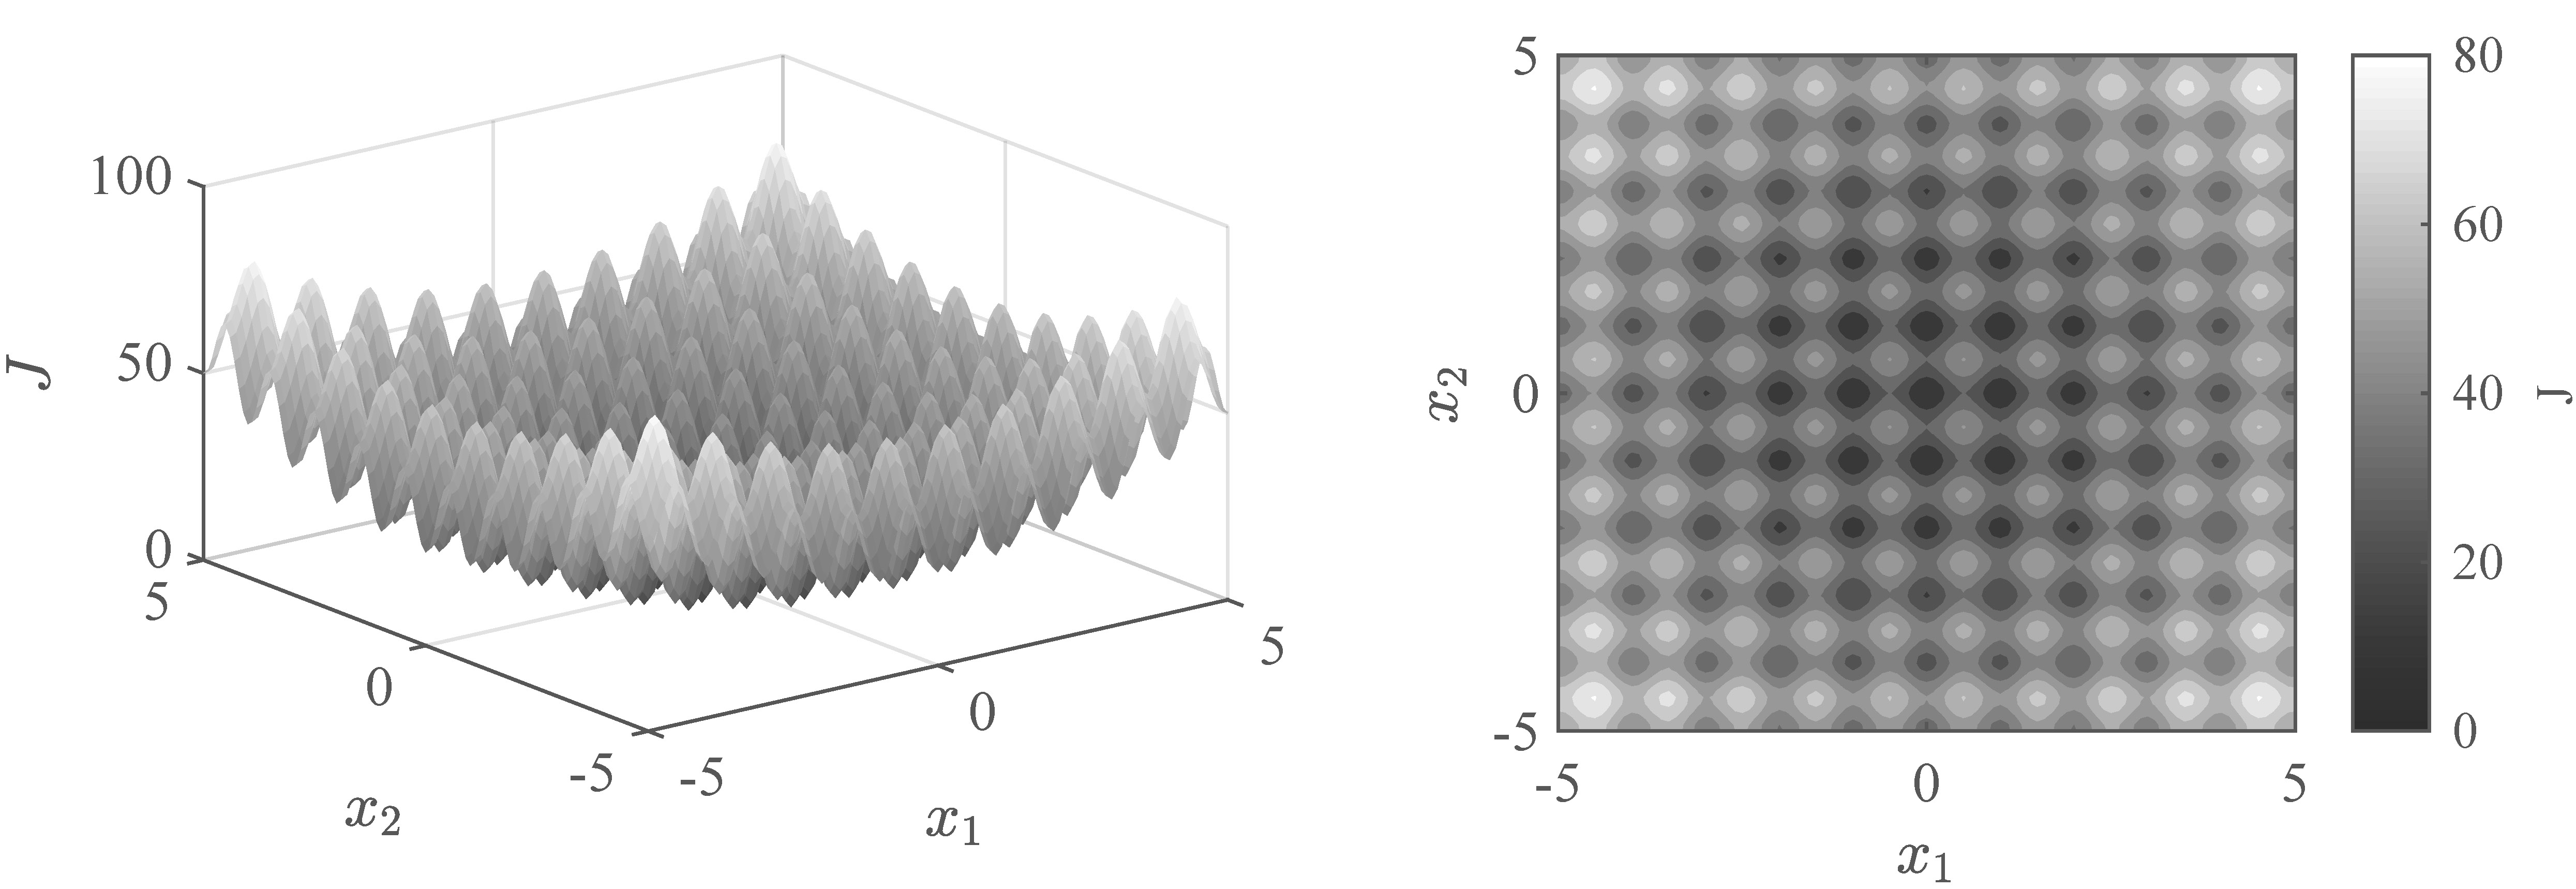
\includegraphics[width=10cm]{fig/lec09/Rastrigin.jpg}
	\label{fig:Rastriging}
	\caption{Rastrigin function $J(\bm{x})=A n + \sum_{i=1}^n \left(x_i^2 - A\cos(2\pi x_i)\right)$ with $A\in\left\{\mathbb{R}|A > 0 \right\}$ as exemplary global optimization problem}
\end{figure}
}

%%%%%%%%%%%%%%%%%%%%%%%%%%%%%%%%%%%%%%%%%%%%%%%%%%%%%%%%%%%%%
%% Possible solutions for the continued use of SGD %%
%%%%%%%%%%%%%%%%%%%%%%%%%%%%%%%%%%%%%%%%%%%%%%%%%%%%%%%%%%%%%
\frame{\frametitle{Possible Solutions for the Continued Use of SGD}
Reinitialize SGD-based learning (multistart approach) e.g.
\begin{itemize}
	\item grid search or
	\item random search (according to some random distribution).
\end{itemize}
\begin{figure}
	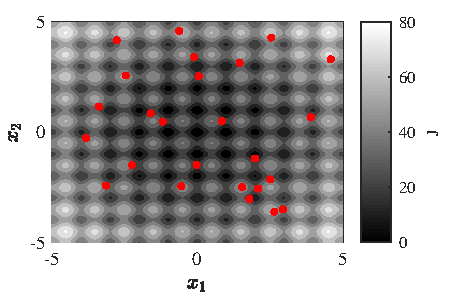
\includegraphics[width=8cm]{fig/lec09/random_search.pdf}
	\label{fig:random_search}
	\caption{Random initialization as one possible tool to find the global optimum in highly non-linear problem spaces}
\end{figure}
}

%%%%%%%%%%%%%%%%%%%%%%%%%%%%%%%%%%%%%%%%%%%%%%%%%%%%%%%%%%%%%
%% Possible Problems With Gradients (2)%%
%%%%%%%%%%%%%%%%%%%%%%%%%%%%%%%%%%%%%%%%%%%%%%%%%%%%%%%%%%%%%
\frame{\frametitle{Possible Problems With Gradients (2)}
What other possible issue may arise when dealing with gradient-based updates?
\begin{itemize}
	\item Depending on the application, one may be forced to use a non differentiable function approximator. 
	\item Close to function singularities, gradients become unfeasibly small or large and cause numeric problems.
\end{itemize}
\begin{figure}
	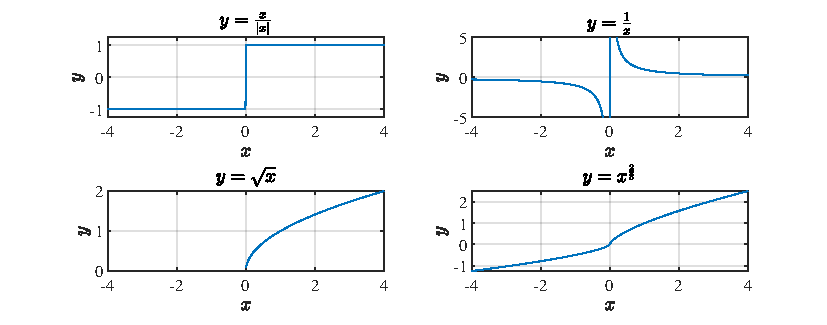
\includegraphics[width=10cm]{fig/lec09/Non_differentiable_functions.pdf}
	\label{fig:Non_differentiable_functions}
	\caption{Examples of non differentiable functions}
\end{figure}
}

%%%%%%%%%%%%%%%%%%%%%%%%%%%%%%%%%%%%%%%%%%%%%%%%%%%%%%%%%%%%%
%% Gradient-free optimization possibilities %%
%%%%%%%%%%%%%%%%%%%%%%%%%%%%%%%%%%%%%%%%%%%%%%%%%%%%%%%%%%%%%
\frame{\frametitle{Gradient-Free Optimization Possibilities}
\onslide<1->{If batch learning is feasible and a consistent data set $\bm{\mathcal{D}}$ is available, gradient-free optimization techniques may become an option like
\begin{itemize}
	\item meta-heuristics such as evolutionary algorithms (EA)  or}
	\onslide<2->{\item surrogate-model-based techniques such as Bayesian optimization.
\end{itemize}}
\onslide<3->{A survey on the taxonomy of cont. global optimization can be found here:
\begin{itemize}
	\item \href{https://arxiv.org/abs/1808.08818}{https://arxiv.org/abs/1808.08818}
\end{itemize}}
\onslide<1->{\begin{figure}
	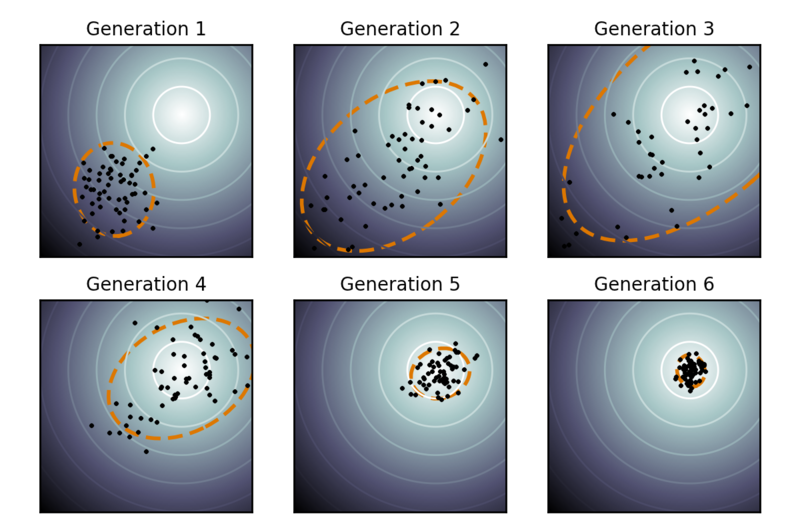
\includegraphics[height=4.25cm]{fig/lec09/EA.png}
	\label{fig:EA}
	\caption{EA iteration examples (source \href{https://en.wikipedia.org/wiki/File:Concept_of_directional_optimization_in_CMA-ES_algorithm.png}{www.wikipedia.org}, \href{https://creativecommons.org/publicdomain/zero/1.0/deed.en}{CC0 1.0})}
\end{figure}}
}

%%%%%%%%%%%%%%%%%%%%%%%%%%%%%%%%%%%%%%%%%%%%%%%%%%%%%%%%%%%%%
%% Summary %%
%%%%%%%%%%%%%%%%%%%%%%%%%%%%%%%%%%%%%%%%%%%%%%%%%%%%%%%%%%%%%
\begin{frame}
\frametitle{Summary: What You've Learned Today}
\begin{itemize}
	\item To cover unfeasible large or continuous state spaces function approximation is required.
	\begin{itemize}\pause
		\item Feature engineering supports the learning process.\pause
	\end{itemize}
	\item On-policy prediction seems rather straightforward with function approximation:
	\begin{itemize}
		\item Just transfer the incremental learning from tabular case to gradient descent on parameter vector $\bm{w}$.\pause
		\item Stochastic gradient descent allows step-by-step based updates.\pause
	\end{itemize}
	\item If bootstrapping is applied, the update target depends on $\bm{w}$.
	\begin{itemize}
		\item True gradient becomes computationally more complex.\pause
		\item Semi-gradient methods reduce computational burden at accuracy costs.\pause
	\end{itemize}
	\item Batch learning squeezes out all available prediction information from a given data set.\pause
	\begin{itemize}
		\item If linear function approximation is applied, closed-form solutions exist.\pause
	\end{itemize}
	\item Gradient-based prediction is not risk free (especially non-linear case):
	\begin{itemize}
		\item no convergence guarantees,
		\item local optima vs. global optimum.
	\end{itemize}
\end{itemize}
\end{frame}

%%%%%%%%%%%%%%%%%%%%%%%%%%%%%%%%%%%%%%%%%%%%%%%%%%%%%%%%%%%%%
%% Final Slide %%
%%%%%%%%%%%%%%%%%%%%%%%%%%%%%%%%%%%%%%%%%%%%%%%%%%%%%%%%%%%%%
\frame{\frametitle{The End for Today}
\vspace{-0.25cm}
\begin{figure}
\hspace*{-0.5cm}

\includegraphics[width=10cm]{fig/lec09/dilbert.jpg}
\end{figure}
\vspace{1cm}
\centering
Thanks for your attention and have a nice week!
}